\chapter{Preliminaries}

% Darstellung der theoretischen Grundlagen
% Definition der verwendeten Begriffe
% allgemeine Konzepte und Ansätze

\section{Intrusion Detection}

Classic security mechanisms, such as encryption or firewalls, are considered as preventive measures for protecting IT infrastructures. However, in order to be able to react to security breaches that have already occurred, additional reactive mechanisms are required. To complement preventive measures, Intrusion Detection Systems (IDSs) have been commercially available since the late 1990s \cite[27]{whitman_principles_2018}.

First, IDSs are described and categorized. In the context of the shortcomings of conventional IDSs for protecting large scale systems, Collaborative Intrusion Detection Systems (CIDSs) are introduced.

\subsection{Intrusion Detection Systems}
Generally, the main reason for operating an IDS is to monitor and analyze computer networks or systems in order to identify anomalies, intrusions or privacy violations \cite{hindy2020taxonomy}. Specifically, the following three advantages are significant \cite[391]{whitman_principles_2018}.

\begin{itemize}
    \item IDSs can detect the preliminaries of attacks, in particular the organized gathering of information about networks and defense mechanisms (attack reconnaissance), and thus enable the prevention or mitigation of damage to information assets.
    \item IDSs can help protect information assets when known vulnerabilities cannot be fixed fast enough, notably in the context of an rapidly changing threat environment.
    \item The occurrence of unknown security vulnerabilities (zero day vulnerabilities) is not predictable, meaning that no specific preparations can be made for them. However, IDSs can identify processes in the IT system that deviate from the normal state and thus contribute to the detection of zero day attacks
\end{itemize}

For an effective IDS, it is important to be able to detect as many steps as possible within the typical attack sequence, also called kill chain \cite[393]{whitman_principles_2018}. Since a successful intrusion into a system can be stopped at several points in this sequence, the effectiveness of the IDS increases with its functionality. The following categorization of intrusion attempts according to \cite{kendall1999database} reflects parts of the kill chain mentioned above:

\begin{description}
    \item[Probing] Probing refers to the preambles of actual attacks, also known as attack reconnaissance. This includes obtaining information about an organization and its network behavior (footprinting) and obtaining detailed information about the used operating systems, network protocols or hardware devices (fingerprinting).
    \item[Denial of Service (DoS)] DoS refers to an attack aimed at disabling a particular service for legitimate users by overloading the target systems processing capacity.
    \item[Remote to Local (R2L)] R2L attacks attempt to gain local access to the target system via a network connection.
    \item[User to Root (U2R)] One step further, U2R attacks start out with user access on the system and gain root access by exploiting vulnerabilities.
\end{description}

Additionally, IDS are generally categorized by the platform being monitored and the employed attack detection method \cite{milenkoski2015evaluating}. Hence, a distinction is made between Host-based Intrusion Detection System (HIDS) and Network-based Intrusion Detection System (NIDS). While a HIDS resides on a system, known as host, only monitoring local activities, a NIDS resides on a network segment and monitors remote attacks that are carried out across the segment. Furthermore, IDS are categorized into signature-based detection and anomaly-based detection. A signature-based IDS (also called knowledge-based detection) compares the system or network state against a collection of signatures of known attacks. The false positive rate is very low when using signatures, but only when assuming the system is confronted with already known attacks. Typically, this method cannot detect novel \cite[403]{whitman_principles_2018}, metamorphic or polymorphic attacks \cite[236]{szor2005art}. An anomaly-based IDS, on the other hand, creates a statistical baseline profile of the system’s or network’s regular state and compares it with the monitored activities. This allows both known and unknown attacks to be detected, but the frequent occurrence of false-positive estimations is a major challenge. Furthermore, hybrid models of the presented approaches from the respective categories exist.

\subsection{Flow Capturing and Network Monitoring}

\subsection{Coordinated Attacks}

\subsection{Collaborative Intrusion Detection Systems}

However, when considering the development of the current threat environment, the effectiveness of conventional intrusion detection systems is limited. Technology trends, such as the internet of things or cloud computing, are main drivers for increasingly blurring corporate boundaries in the context of interconnection of infrastructures and shared resources. This transformation increases the potential attack surface of productive computer systems for large-scale and high-velocity cyber attacks, which traditional IDSs have limited effectiveness due to their isolated nature. For example, such stand-alone IDS will not be able to create connections between security events that occur at different infrastructures simultaneously. Due to the mentioned increase of attack surface that is related to the size of current computer networks, attackers may attempt to obfuscate the characteristic overall sequence of the intrusion by spreading single attack steps.

n order to address the aforementioned security problems of large IT systems, Collaborative Intrusion Detection Systems (CIDSs) have been proposed. In general, a CIDS is a network of several intrusion detection components that collect and exchange data on system security. A CIDS is essentially specified by two different types of components, namely the detection units and the correlation units, and their communication among each other. The detections units can be considered as conventional IDS that monitor a sub-network or a host and by that, generate low-level intrusion alerts. The correlation unit is responsible for merging the low-level intrusion alerts and their further post-processing. This includes, for instance, the correlation of the alerts, the generation of reports or the distribution of the information to the participants of the network. CIDSs pursue the following two goals \cite[24]{vasilomanolakis_collaborative_2016}.

\begin{itemize}
    \item The aggregation and correlation of data originating from different IDSs creates a holistic picture of the network to be monitored and enables the detection of distributed and coordinated attacks.
    \item CIDSs can monitor large-scale networks more effectively with the realization of a loadbalancing strategy. By sharing IDS resources across different infrastructures, short-term peak loads can be served, reducing the downtime of individual IDSs.
\end{itemize}
\newpage
\section{Gaussian Mixture Models}

This section focuses the concept of \acrshort{gmm} for density estimation. For this purpose, the Gaussian normal distribution is presented first, by introducing basic definitions for the probability density functions and describing the closure properties of the distribution. For this purpose, at the beginning a short motivation for the application of the presented model will be given. Then, mixture models in general and \acrshort{gmm} in particular are defined. After that, two main concepts will be explained. First, the \acrshort{gmm} is interpreted in terms of a \acrshort{lvm}. Second, the \acrshort{ema} is presented, which performs the computation of model parameters of latent variable models in an iterative scheme.

\subsection{Gaussian Distribution}

The Gaussian normal distribution forms the basic building block for \acrshort{gmm}s. Depending on the observed random variable, different types of normal distributions exist. In particular, the multivariate normal distribution is focused on when considering statistical flow features, which are typically continuous and high dimensional. In the following, different definitions for the normal distribution are introduced and important properties are presented that are essential for calculations during the learning phase of \acrshort{gmm}s.

Let be a multivariate random variable $\bm{X} = (X_1, \dots, X_D)^T$, where each element $X_d$ with $d \in \{1, \dots, D\}, D \in \mathbb{N}$ is a univariate random variable that follows a normal distribution, which is referred to as $X_d \sim \mathcal{N}(\mu, \sigma^2)$.

\begin{definition}[Univariate Gaussian Distribution] \cite[p. 175]{dei_2020}
A continuous, univariate random variable $X$ is said to follow a normal distribution, if it exhibits a probability density function
\begin{equation*}
p(x | \mu, \sigma^2) = \frac{1}{\sqrt{2\pi \sigma^2}} exp\bigg(- \frac{(x-\mu)^2}{2\sigma^2}\bigg),
\end{equation*}
\end{definition}

with $x \in \mathbb{R}$ and where $\mu$ refers to the mean and $\sigma^2$ is the variance of the distribution. Then, if $\bm{X}$ follows a normal distribution, this is expressed as a multivariate Gaussian distribution, denoted by $\bm{X} \sim \mathcal{N}_D(\bm{\mu}, \bm{\Sigma})$, which is fully described by its mean vector $\bm{\mu}$ and its covariance matrix $\bm{\Sigma}$.

\begin{definition}[Multivariate Gaussian Distribution]\label{def:multivariate_pdf} \cite[175]{dei_2020}
A multivariate random variable $\bm{X}$ follows a normal distribution, if it is described by a probability density function
\begin{equation*}
    p(\bm{x} | \bm{\mu}, \bm{\Sigma}) = (2\pi)^{-\frac{D}{2}} |\bm{\Sigma}|^{-\frac{1}{2}}exp\left(-\frac{1}{2}(\bm{x}-\bm{\mu})^T \bm{\Sigma}^{-1}(\bm{x}-\bm{\mu})\right),
\end{equation*}
\end{definition}

with $\bm{x} \in \mathbb{R}^D$. The mean vector specifies the estimate of the expected value of the distribution, with each of its components describing the mean $\mu$ of the corresponding dimension. The empirical covariance $\bm{\Sigma}$ models the estimate of the variance along each dimension as well as the correlation between the different dimensions. The diagonal elements of $\bm{\Sigma}$ describe the variance of the random variable corresponding to the respective dimension and the off-diagonal elements describe the covariance relationship between the respective random variables. 

An illustration of the influence of the described parameters on the location and shape of a multivariate distribution is given in Figure \ref{fig:multiple_bivariate}. Specifically, three bivariate normal distributions are considered, whose random variables each have different values with respect to their correlation, while the mean vector is the same for all distributions.
 
\begin{figure}%
    \centering%
    \begin{subfigure}[b]{0.25\textwidth}%
        \centering\captionsetup{width=.8\linewidth}%
        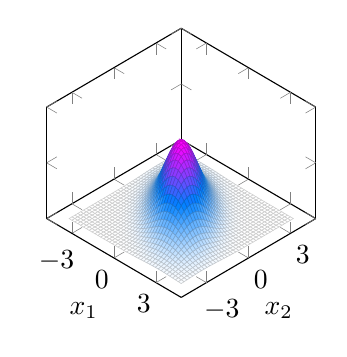
\begin{tikzpicture}
  \def\p{-0.6}%
  \def\centerx{0}%
  \def\centery{0}%
  \pgfplotsset{
      colormap={cool}{rgb255(0cm)=(255,255,255); rgb255(1cm)=(0,128,255); rgb255(2cm)=(255,0,255)}
  }%
    \begin{axis}[
      width=5cm,height=5cm,
      xlabel=$x_1$,
      ylabel=$x_2$,
      xlabel shift={-10pt},
      ylabel shift={-10pt},
      zmin=0,
      zmax=0.2,
      domain=-4:4,
      enlarge x limits,
      enlarge y limits,
      scaled y ticks=false,
      scaled x ticks=false,
      xtick={-3, 0, 3},
      xticklabels={$-3$, $0$, $3$},
      ytick={-3, 0, 3},
      yticklabels={$-3$, $0$, $3$},
      zticklabels={},
      view={45}{45},
      % colorbar horizontal,
      colormap name=cool,
      % colorbar style={
      %   xtick={0, 0.05, 0.1, 0.15, 0.2},
      %   xticklabels={$0$, $0.05$, $0.1$, $0.15$, $0.2$},
      % }
      ]%
      \addplot3[surf, samples=40, shader=faceted, very thin]
      {1/(2 *pi* sqrt(1-\p^2))* exp(-((x-\centerx)^2+(y-\centery)^2-2*\p*(x-\centerx)*(y-\centery))/(2*(1-\p^2))};%
    \end{axis}
\end{tikzpicture}%
        \caption{}%
        \label{subfig:bivariate_neg}%
    \end{subfigure}%
    % \hfill%
    \begin{subfigure}[b]{0.33\textwidth}%
        \centering\captionsetup{width=.8\linewidth}%
        \def\p{0.0}%
\def\centerx{0}%
\def\centery{0}%
\pgfplotsset{
    colormap={cool}{rgb255(0cm)=(255,255,255); rgb255(1cm)=(0,128,255); rgb255(2cm)=(255,0,255)}
}%
\begin{tikzpicture}
    \begin{axis}[
      width=5cm,height=5cm,
      xlabel=$x_1$,
      ylabel=$x_2$,
      xlabel shift={-10pt},
      ylabel shift={-10pt},
      zmin=0,
      zmax=0.2,
      domain=-4:4,
      enlarge x limits,
      enlarge y limits,
      scaled y ticks=false,
      scaled x ticks=false,
      xtick={-3, 0, 3},
      xticklabels={$-3$, $0$, $3$},
      ytick={-3, 0, 3},
      yticklabels={$-3$, $0$, $3$},
      zticklabels={},
      view={45}{45},
      % colorbar horizontal,
      colormap name=cool,
      % colorbar style={
      %   xtick={0, 0.05, 0.1, 0.15, 0.2},
      %   xticklabels={$0$, $0.05$, $0.1$, $0.15$, $0.2$},
      % }
      ]%
      \addplot3[surf, samples=40, shader=faceted,thin]
      {1/(2 *pi* sqrt(1-\p^2))* exp(-((x-\centerx)^2+(y-\centery)^2-2*\p*(x-\centerx)*(y-\centery))/(2*(1-\p^2))};%
    \end{axis}
\end{tikzpicture}%
        \caption{}%
        \label{subfig:bivariate_neutral}%
    \end{subfigure}%
    % \hfill%
    \begin{subfigure}[b]{0.33\textwidth}%
        \centering\captionsetup{width=.8\linewidth}%
        \def\p{0.6}%
\def\centerx{0}%
\def\centery{0}%
\pgfplotsset{
    colormap={cool}{rgb255(0cm)=(255,255,255); rgb255(1cm)=(0,128,255); rgb255(2cm)=(255,0,255)}
}%
\begin{tikzpicture}
    \begin{axis}[
      width=5cm,height=5cm,
      xlabel=$x_1$,
      ylabel=$x_2$,
      xlabel shift={-10pt},
      ylabel shift={-10pt},
      zmin=0,
      zmax=0.2,
      domain=-4:4,
      enlarge x limits,
      enlarge y limits,
      scaled y ticks=false,
      scaled x ticks=false,
      xtick={-3, 0, 3},
      xticklabels={$-3$, $0$, $3$},
      ytick={-3, 0, 3},
      yticklabels={$-3$, $0$, $3$},
      zticklabels={},
      view={45}{45},
      colorbar,
      colormap name=cool,
      colorbar style={
        title={$p(x_1, x_2)$},
        ytick={0, 0.1, 0.197},
        yticklabels={$0.0$, $0.1$, $0.2$},
        height=2.8cm,
        at={(1.1,0)},
        anchor=south west
        % ylabel=$p(x_1, x_2)$
      },
      colorbar/width=2.5mm,
      ]%
      \addplot3[surf, samples=40, shader=faceted,thin]
      {1/(2 *pi* sqrt(1-\p^2))* exp(-((x-\centerx)^2+(y-\centery)^2-2*\p*(x-\centerx)*(y-\centery))/(2*(1-\p^2))};%
    \end{axis}
\end{tikzpicture}%
        \caption{}%
        \label{subfig:bivariate_pos}%
    \end{subfigure}%
    \caption{Bivariate gaussian distributions exhibit different shapes with a changing correlation value between the random variables $x_1$ and $x_2$: (\subref{subfig:bivariate_neg}) negative, (\subref{subfig:bivariate_neutral}) zero and (\subref{subfig:bivariate_pos}) positive correlation}%
    \label{fig:multiple_bivariate}%
\end{figure}%

Having introduced the basic definition of Gaussian distributions, it is now examined how they can be manipulated to obtain information necessary for parameter learning of Gaussian mixture models. Two practical algebraic properties of normal distributions, namely closure under \textit{conditioning} and \textit{marginalization} are detailed for this purpose. Being closed under conditioning and marginalization in this case means that when one or more components of a Gaussian distribution is marginalized out or conditioned on, that the resulting distribution is still Gaussian. This not only distinguishes Gaussian distributions from other distributions, but also makes them easier to handle mathematically. Since both marginalization and conditioning act on subsets of the original distribution, the following notation is introduced first. Considering a multivariate Gaussian random variable $\bm{X} \sim \mathcal{N}(\bm{\mu}, \bm{\Sigma})$, we partition $\bm{X}$ according to 

\begin{equation*}
    \bm{X} = \left[ \begin{array}{c}
        \bm{X}_M \\
        \bm{X}_N
    \end{array} \right],
\end{equation*}

with $\bm{X}_M \in \mathbf{R}^M$, where $M < N$, and $\bm{X}_N \in \mathbf{R}^N$, where $N=D-M$. In general, $\bm{X}_M$ is chosen to be the first $M$ elements of $\bm{X}$ and $\bm{X}_N$ the rest. Accordingly, $\bm{\mu}$ and $\bm{\Sigma}$ are partitioned as
\begin{equation*}
    \left[ \begin{array}{c}
        \bm{X}_M \\
        \bm{X}_N
    \end{array} \right] \sim \mathcal{N} \left( \left[\begin{array}{c}
         \bm{\mu}_M \\
         \bm{\mu}_N
    \end{array}\right], \left[\begin{array}{cc}
        \bm{\Sigma}_{MM} & \bm{\Sigma}_{MN} \\
        \bm{\Sigma}_{NM} & \bm{\Sigma}_{NN}
    \end{array}\right] \right).
\end{equation*}

With this form, it is now possible to express the extraction of partial information from multivariate probability distributions by means of marginalization. 

\begin{definition}[Marginal of a Gaussian Distribution]\label{def:marg_gaussian} \cite[p. 177]{dei_2020}
Given $\bm{X} \sim \mathcal{N}_D(\bm{\mu}, \bm{\Sigma})$, with partitions $\bm{X}_M, \bm{X}_N$, the distributions of $\bm{X}_M$ and $\bm{X}_N$ are called marginals and their corresponding probability density function can be obtained by
\begin{equation*}
    p(\bm{x}_M) = \int p(\bm{x}_M,\bm{x}_N)d\bm{x}_N.
\end{equation*}
\end{definition}

Furthermore, each partition $\bm{X}_M, \bm{X}_N$ only depend on its corresponding entries in $\bm{\mu}$ and  $\bm{\Sigma}$, which leads to the following theorem. 

\begin{theorem} \cite[p. 177]{dei_2020}
The marginal distribution of a Gaussian distribution is also a Gaussian and determined by
\begin{equation*}
    \bm{X}_M \sim \mathcal{N}(\bm{\mu}_M, \bm{\Sigma}_{MM}).
\end{equation*}
\end{theorem}

The conditional Gaussian is typically utilized in the context of posterior distributions, such as in the process of density estimation of \acrshort{gmm}s, and is defined as follows.

\begin{definition}[Conditional of a Gaussian Distribution] \cite[p. 177]{dei_2020}
Given $\bm{X} \sim \mathcal{N}_D(\bm{\mu}, \bm{\Sigma})$, with partitions $\bm{X}_M, \bm{X}_N$, the conditional distribution is defined as
\begin{align*}
    p(\bm{x}_M | \bm{x}_N) &= \mathcal{N}(\bm{\mu}_{M | N}, \bm{\Sigma}_{M | N}), \\
    \bm{\mu}_{M | N} &= \bm{\mu}_M + \bm{\Sigma}_{M N} + \bm{\Sigma}^{-1}_{N N}(\bm{x}_N - \bm{\mu}_N),\\
    \bm{\Sigma}_{M | N} &= \bm{\Sigma}_{M M} - \bm{\Sigma}_{M N} \bm{\Sigma}^{-1}_{N N}\bm{\Sigma}_{N M}.\\
\end{align*}
\end{definition}

\begin{theorem} \cite[p. 177]{dei_2020}
The conditional distribution of a Gaussian distribution is also a Gaussian and defined by 
\begin{equation*}
    \bm{X}_{M | N} \sim \mathcal{N}(\bm{\mu}_{M | N}, \bm{\Sigma}_{M | N}).
\end{equation*}
\end{theorem}

A line of arguments proving the stated theorems can be found in section 2.3 in \cite{bis_2006}.

% \begin{figure}[b]
%     \centering
%     % \documentclass{standalone}

% \usepackage{pgfplots}

% \begin{document}
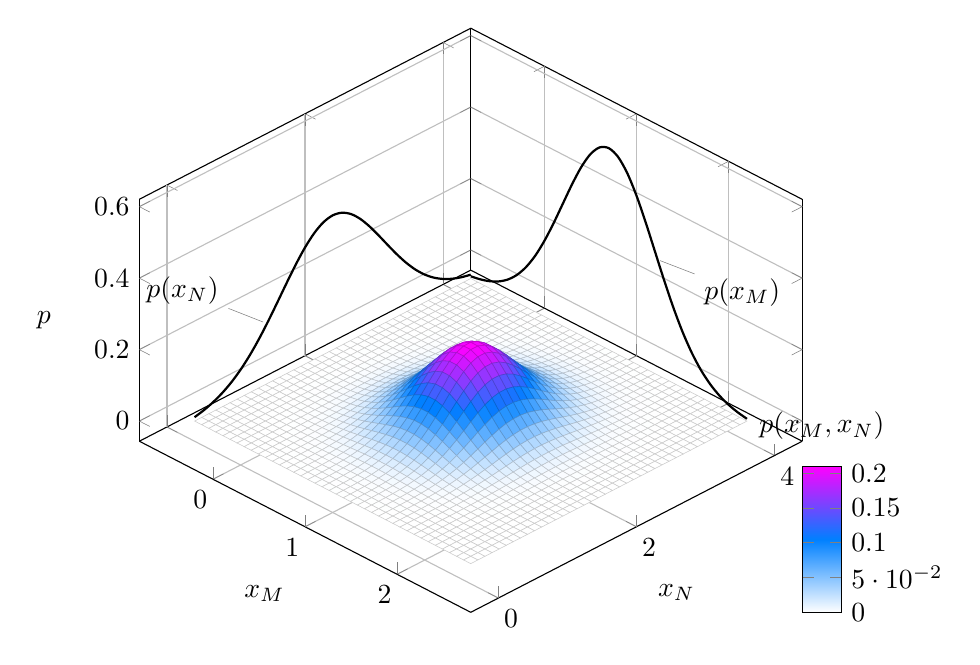
\begin{tikzpicture}[
    declare function={mu1=1;},
    declare function={mu2=2;},
    declare function={sigma1=0.5;},
    declare function={sigma2=0.75;},
    declare function={normal(\m,\s)=1/(2*\s*sqrt(pi))*exp(-(x-\m)^2/(2*\s^2));},
    declare function={bivar(\ma,\sa,\mb,\sb)=
        1/(2*pi*\sa*\sb) * exp(-((x-\ma)^2/\sa^2 + (y-\mb)^2/\sb^2))/2;}]
    \pgfplotsset{colormap={cool}{rgb255(0cm)=(255,255,255); rgb255(1cm)=(0,128,255); rgb255(2cm)=(255,0,255)}}%
\begin{axis}[
    colormap name=cool,
    width=10cm, height=9cm,
    view={45}{45},
    enlarge x limits,
    enlarge y limits,
    grid=major,
    domain=-0.5:2.5,
    y domain=0:4,
    ymin=0,
    ymax=4,
    xmin=-0.5,
    xmax=2.5,
    samples=40,
    xlabel=$x_M$,
    ylabel=$x_N$,
    zlabel={$p$},
    every axis z label/.style={rotate=0, at={(current axis.west)}, left=10mm},
    colorbar,
    colorbar style={
        at={(1,0)},
        anchor=south west,
        height=0.25*\pgfkeysvalueof{/pgfplots/parent axis height},
        title={$p(x_M,x_N)$}
    }
]
\addplot3 [surf, shader=faceted, very thin] {bivar(mu1,sigma1,mu2,sigma2)};
\addplot3 [domain=-0.5:2.5,samples=31, samples y=0, thick, smooth] (x,4,{normal(mu1,sigma1)});
\addplot3 [domain=0:4,samples=31, samples y=0, thick, smooth] (-0.5,x,{normal(mu2,sigma2)});
% \addplot3 [domain=0:4,samples=31, samples y=0, thick, smooth] (x,2,{normal(mu1,0.95)});
\node at (axis cs:-0.4,1,0.18) [pin=165:$p(x_N)$] {};
\node at (axis cs:1.45,4,0.32) [pin=-15:$p(x_M)$] {};
\end{axis}
\end{tikzpicture}
% \end{document}
%     \caption{Cryptographic hash function and locality-sensitive hash function exhibit different properties for the probability of collisions.}
%     \label{fig:hashing_differences}
% \end{figure}

% \begin{figure}[ht!]
% \begin{example}{Examples on the closure properties of Gaussians}{closure_examples}

% Considering the random variable $\bm{X}_a$ from Example \ref{ex:bivariate_gaussian}, the marginalization and conditioning operations are applied and the respective results are visualized . \\

% First, $\bm{X}_a$ is partitioned as
% \begin{equation*}
%     \bm{X}_a = 
%     \left[ \begin{array}{c}
%         X_M \\
%         X_N
%     \end{array} \right] \sim \mathcal{N} \left( \left[\begin{array}{c}
%          0 \\
%          0
%     \end{array}\right], \left[\begin{array}{cc}
%         1.5 & -1.0 \\
%         -1.0 & 0.75
%     \end{array}\right] \right).
% \end{equation*}

% The marginal distributions can be obtained by taking the corresponding values directly from the original distribution, which are
% \begin{align*}
%     p(x_M) = \mathcal{N}(0, 1.5), \\
%     p(x_N) = \mathcal{N}(0, 1.5).
% \end{align*}

% Now, the conditional distribution $p(\bm{x}_M | \bm{x}_N)$ for $\bm{x}_N = 1$ is obtained as
% \begin{align*}
%     \overline{x}_{M | N} &= 0 - 1 + \frac{1}{0.75} \cdot (1-0) = \frac{1}{3}\\
%     \sigma^2_{M | N} &= 1.5 + \frac{1}{0.75} = \frac{17}{6}  \\
%     p(x_{M | N}) &= \mathcal{N}\left(\frac{1}{3} , \frac{17}{6}\right).
% \end{align*}

% \vspace{1cm}

% \begin{minipage}{0.65\textwidth}
%     \centering
%         \begin{subfigure}[t]{\linewidth}
%         \centering
%         \includegraphics[width=0.99\linewidth]{figures/joint_gaussian.png}
%         \subcaption{}
%         \label{fig:joint_gaussian_with_marg}

%         \end{subfigure}
% \end{minipage}
% \begin{minipage}{0.34\textwidth}
%     \centering
%     \begin{subfigure}[t]{\linewidth}
%         %\centering
        
%         \includegraphics[width=0.99\linewidth]{figures/contour_gaussian_conditioned_example.png}
%         \subcaption{}
%         \label{fig:contour_cond_gaussian}
%     \end{subfigure}
%     \begin{subfigure}[t]{\linewidth}
%         %\centering
%         \includegraphics[width=0.99\linewidth]{figures/cond_gaussian.png}
%         \subcaption{}
%         \label{fig:cond_gaussian}
        
%     \end{subfigure}
% \end{minipage}
% \caption[Plots of a joint Gaussian distribution and its corresponding marginal and conditional distributions]{The 3D-plot on the left (\ref{fig:joint_gaussian_with_marg}) shows the joint distribution $p(x_M, x_N)$ with their corresponding marginals. The contour plot on the upper right (\ref{fig:contour_cond_gaussian}) visualizes $p(x_M, x_N)$ with the conditioning value. The plot on the lower right (\ref{fig:cond_gaussian}) illustrates the conditional distribution $p(x_M | x_N)$ with $x_N=1$.}
% \end{example}
% \end{figure}

\newpage
% \input{2_mainmatter/2_theoretical_background/2_2_density_estimation.tex}

\subsection{Gaussian Mixtures}

In this section, the \acrshort{gmm} is presented as a model for density estimation. For this purpose, at the beginning a short motivation for the application of the presented model will be given. Then, mixture models in general and \acrshort{gmm} in particular are defined. After that, two main concepts will be explained. First, the \acrshort{gmm} is interpreted in terms of a \acrshort{lvm}. Second, the \acrshort{ema} is presented, which performs the computation of model parameters of latent variable models in an iterative scheme.

\subsubsection{Motivation}
Using statistical estimation techniques, it is possible to estimate an unobservable underlying probability density function from observed data. This allows data to be compactly represented with a density from a parametric family, such as a Gaussian distribution. However, all conventional parametric distributions are limited in their modeling capabilities when confronted with real data. For example, looking at the marginal distribution $p(x_1)$ in Figure \ref{fig:multimodal_dataset}, it is apparent that the data follow a multimodal distribution, i.e., have more than one center. A density estimate using a simple Gaussian distribution is not sufficient to effectively represent such multimodal data. Therefore, a more flexible type of distribution needs to be introduced that can be used for density estimation.

% \begin{figure}[h]
%     \centering
%     \includegraphics[width=0.8\textwidth]{figures/gaussian_example_dataset.pdf}
%     \caption[Illustration of an exemplary dataset with two dimensions exhibiting a multimodal distribution]{This figure illustrates an examplary dataset with two dimensions. Within the center of this figure, there is a scatter plot showing the observed data points $\bm{x} \in \bm{X}$. At the bottom and right edge of the scatter plot, there are histograms showing the marginal distributions of the dataset.}
%     \label{fig:multimodal_dataset}
% \end{figure}

\subsubsection{Definition}

The idea is to represent a multimodal distribution by constructing a linear combination of multiple simple distributions, each of which representing a unimodal sub-population of the data, which is formalized under the term \textit{mixture model} \cite[p.111]{bis_2006}.

\begin{definition}[Mixture Model] \cite[p. 315]{dei_2020}
A mixture model is a linear combination of $K$ parametric distributions $p_k$, each weighted by a mixture weight $\pi_k$, with the following form 
\begin{align*}
    &p(x) = \sum\limits_{k=1}^K \pi_k p_k (x), \\
    &0 \leq \pi_k \leq 1, \sum\limits_{k=1}^K \pi_k = 1.
\end{align*}
\end{definition}

A distribution $p_k$ within this model is called mixture component and the sum of the mixture weights equals to 1, such that the probability density of the mixture components equals to 1 as well. 

Mixture Models can use any arbitrary parametric distribution as component density, but the most common mixture model is the Gaussian mixture model, using Gaussians as components \cite[214]{has_2009}. First, \acrshort{gmm}s utilize the practical mathematical properties of Gaussians, introduced earlier in Section \ref{sec:gaussian_distribution}. Furthermore, the quality of the model, in terms of its ability to estimate real data distributions, is theoretically supported by the Central Limit Theorem, which states, that most data distributions converge to a normal distribution on average as the number of data points increases (see \cite[p.222]{jay_2003} for a proof).

\begin{theorem}[Central Limit Theorem]\label{th:central_limit} \cite[p.241]{montgomery_2010}
Consider $N$ i.i.d. random variables $X_i$ with $\mathrm{E}[X_i]=\overline{x}$ and $\mathrm{var}[X_i]=\sigma^2$ and let $S_N=\sum^N_{i=1}X_i$. It can be shown that, as $N$ increases, that
\begin{equation*}
    p(S_N) \sim \mathcal{N}\left(\overline{x}, \frac{\sigma^2}{N}\right).
\end{equation*}
\end{theorem}

\begin{definition}[Gaussian Mixture Model]\label{def:gmm} \cite[p. 315]{dei_2020}
A \acrlong{gmm} is a combination of a finite number of $K$ Gaussian distributions $\mathcal{N}(\bm{x}|\theta_k)$ which is fully described by a probability density function $p$ and its parameter set $\theta$ as
\begin{equation}\label{eq:gmm_def}
    \begin{aligned}
        &p(\bm{x}|\theta) = \sum\limits_{k=1}^K \pi_k \mathcal{N}(x | \theta), \\
        &0 \leq \pi_k \leq 1, \sum\limits_{k=1}^K \pi_k = 1, \\
        &\theta := \{\overline{\bm{x}}_k, \bm{\mathrm{C}}_k, \pi_k : k = 1, \dots, K \}.
    \end{aligned}
\end{equation}
\end{definition}

% \begin{figure}[h!]
% \begin{example}{Gaussian Mixture Model with three components}{gmm_examples}

% This example illustrates a \acrshort{gmm} with three components that has been fitted to the dataset shown in Figure \ref{fig:multimodal_dataset}.

% \begin{equation*}
%         p(\bm{x}|\theta) = \sum\limits_{k=1}^{3}\pi_k\mathcal{N}(x|\overline{\bm{x}}_k, \bm{\mathrm{C}}_k)
% \end{equation*}

% \begin{equation*}
% \setlength{\jot}{10pt}
%     \begin{aligned}
%     k = 1:& \quad \pi_1=0.23, \; p_1(\bm{x})=\mathcal{N} \left( \left[\begin{array}{c}
%          3.00 \\
%         -4.68
%     \end{array}\right], \left[\begin{array}{cc}
%         0.57 & -0.41 \\
%         -0.41 & 0.66
%     \end{array}\right] \right)\\
%     k = 2:& \quad  \pi_2=0.33 \; p_2(\bm{x})=\mathcal{N} \left( \left[\begin{array}{c}
%          0.30 \\
%         -6.34
%     \end{array}\right], \left[\begin{array}{cc}
%         0.75 & 0.68 \\
%         0.68 & 1.45
%     \end{array}\right] \right)\\
%     k = 3:& \quad \pi_3=0.44 \; p_3(\bm{x})=\mathcal{N} \left( \left[\begin{array}{c}
%          5.36 \\
%         -5.29
%     \end{array}\right], \left[\begin{array}{cc}
%         0.67 & 0.31 \\
%         0.31 & 0.85
%     \end{array}\right] \right)\\
%     \end{aligned}
% \end{equation*}

%     \begin{subfigure}[ht]{0.66\textwidth}
%         \centering
%         \includegraphics[width=\textwidth]{figures/example_dataset_gmm_3d.png}
%         \caption{}
%         \label{fig:gmm_ex_joint}
%     \end{subfigure}
%     \hfill
%     \begin{subfigure}[ht]{0.33\textwidth}
%         \centering
%         \includegraphics[width=\textwidth]{figures/example_dataset_contour_gmm.png}
%         \caption{}
%         \label{fig:gmm_ex_contour}
%     \end{subfigure}
%     \label{fig:contour_gaussian}
%     \caption[Plots of a Distribution according to a Gaussian Mixture Model]{Both plots visualize a Gaussian Mixture Model that has been fitted to the exemplary dataset from Figure \ref{fig:multimodal_dataset}. Unlike a simple distribution, the mixture model is capable of representing multimodal data.}

% \end{example}
% \end{figure}

\subsubsection{Probabilistic Modeling}
So far, with the definition and the example, an intuitive explanation of the \acrshort{gmm} has been given. Before it is explained how to estimate the parameters of the model, it is necessary to look at the subject from the perspective of probabilistic modeling. Probabilistic models, in general, utilize the mathematics of probability theory in order to express all forms of uncertainty and noise that is associated with the learning task. If a Bayesian interpretation is thereby applied to the probabilities, then this is commonly referred to as Bayesian Inference. This allows, for example, the estimation of the parameters of a probability distribution or a statistical model utilizing Bayes' Theorem \cite[p.245]{dei_2020}. 

In this case, discrete latent variables must be introduced into the construction, which allows a probabilistic model to be formed by defining a joint distribution over observed variables and latent variables \cite[432]{bis_2006}. 

The term latent variable usually refers to a variable that cannot be observed directly, but can be inferred from other observable variables using mathematical models \cite{bor_2003}. Models involving such latent variables, called \acrshort{lvm}, are usually harder to fit than models without latent variables, but often have fewer parameters due to their natural implication of a bottleneck, resulting in a compressed representation of the data \cite[337]{mur_2012}. 

For simplicity, first a single data point $\bm{x}$ is considered, which is later expanded to a set of data points $\bm{X}:=\{\bm{x}_1, \dots, \bm{x}_N\}$. It is further assumed a \acrshort{gmm} with $K$ components. Thus, a $K$-dimensional binary random variable $\bm{z}$ is introduced, that indicates whether the $k$th mixture component is responsible for generating the data point $\bm{x}$. Hence, only a particular element $z_k$ is equal to one and all other elements are equal to zero, such that

\begin{equation}
    z_k \in \{0,1\}, \quad \sum\limits^K_{k=1} z_k=1.
\end{equation}

For the construction of a probabilistic model, it is necessary to specify the joint distribution of the observed data $\bm{x}$ and the latent variable $\bm{z}$. Therefore, the factors of the joint distribution are defined as

\begin{equation}\label{eq:joint_lat_var}
    p(\bm{x},\bm{z}) = p(\bm{z})p(\bm{x}|\bm{z}).
\end{equation}

The responsibility of mixture component $k$ generating a data point $\bm{x}$ can be expressed as the conditional distribution of $\bm{x}$ given a specific assignment for $\bm{z}$, which is a Gaussian

\begin{equation}\label{eq:cond_lat_var}
    p(\bm{x} | z_k=1) = \mathcal{N}(\bm{x} | \overline{\bm{x}}_k, \bm{\mathrm{C}}_k) \quad \Rightarrow \quad p(\bm{x}|\bm{z}) = \prod\limits^K_{k=1}\mathcal{N}(\bm{x} | \overline{\bm{x}}_k, \bm{\mathrm{C}}_k)^{z_k} .
\end{equation}

In practice, there exists no knowledge about the value assignment of the latent variables. Therefore, a prior is set to $\bm{z}$, which is defined as

\begin{equation}\label{eq:prior_lat_var}
    p(\bm{z})=\bm{\pi}=[\pi_{1}, \dots, \pi_{K}]^T = \prod\limits^K_{k=1}\pi_k^{z_k}, \quad \sum\limits_{k=1}^K\pi_{k}=1.
\end{equation}

Now, there is a way to describe the \textit{probability} that the $k$th mixture component generated the data point $\bm{x}$ as

\begin{equation}
    p(z_k=1)=\pi_k.
\end{equation}

% \begin{figure}[h]
%   \begin{minipage}[t]{0.4\textwidth}
%   \vspace{0pt}
%   \centering
%     \caption[A Gaussian Mixture Model represented in plate notation]{
%        Both graphs represent a \acrshort{gmm} using plate notation. While the left graph (a) includes a single data point $\bm{x}$, the graph on the right side (b) extends the model to a full dataset with $N$ i.i.d. data points $\{\bm{x}_n\}$ and corresponding latent variables $\{\bm{z}_n\}$. Note, that the directed edge from the latent variable to the observed data reflects the joint distribution from (\ref{eq:joint_lat_var}).
%     }\label{fig:gmm_plate_notation}
%   \end{minipage}
%   \hfill
%   \begin{minipage}[t]{0.25\textwidth}
%   \vspace{0pt}
%     \begin{tikzpicture}
    \node[obs] (x) {$\bm{x}$};
    \node[latent, above= of x] (z) {$\bm{z}$};
    \node[above=of z] (pi) {$\bm{\pi}$};
    
    \node[left=of x] (cov) {$\bm{\mathrm{C}}_k$};
    \node[above=of cov, yshift=-1cm] (mean) {$\overline{\bm{x}}_k$};
    
    \plate {plate1} {(mean)(cov)} {$k=1, \dots, K$};
    
    \edge{pi}{z};
    \edge{z}{x};
    \edge{mean}{x};
    \edge{cov}{x}
    
    
    \end{tikzpicture}
%     \centering
%     \vspace{2.5pt}
%     (a)
%   \end{minipage}
%   \hfill
%   \begin{minipage}[t]{0.285\textwidth}
%   \vspace{0pt}
%     \subfile{tikz/plate_multi_point.tex}
%     \centering
%     \vspace{2.5pt}
%     (b)
%   \end{minipage}
% \end{figure}

Then the conditional distribution $p(\bm{x}|\bm{z})$ from (\ref{eq:cond_lat_var}) and the prior distribution $p(\bm{z})$ from (\ref{eq:prior_lat_var}) are plugged into the joint distribution $p(\bm{z})p(\bm{x}|\bm{z})$ from (\ref{eq:joint_lat_var}) and the marginal distribution $p(\bm{x})$ is obtained by summing the joint distribution over all possible states of $\bm{z}$, which results in 

\begin{equation}\label{eq:joint_marg_lat_var}
    p(\bm{x}) = \sum\limits_{\bm{z}}p(\bm{z})p(\bm{x}|\bm{z}) = \sum\limits_{k=1}^K\pi_k\mathcal{N}(\bm{x} | \overline{\bm{x}}, \bm{\mathrm{C}}).
\end{equation}

It can be confirmed that the \acrshort{gmm} has been extended by including the discrete latent variable  $\bm{z}$ and that the result is still consistent with the previous definition, since the marginal distribution $p(\bm{x})$ is a Gaussian mixture of the form (\ref{eq:gmm_def}). This enables the joint distribution $p(\bm{x}, \bm{z})$ to be used in place of the marginal distribution $p(\bm{x})$, greatly simplifying parameter estimation by applying the \acrshort{ema}.

So far, it was assumed that the dataset consists of a single data point $\bm{x}$. Now, the dataset is extended to $N$ data points that can be denoted by the matrix $\bm{X} \in \mathbb{R}^{N \times D}$. From that, it follows that every data point $\bm{x}_n$ possesses its own latent variable $\bm{z}_n$. Similarly, all latent variables can be summarized by the matrix $\bm{Z} \in \mathbb{R}^{N \times K}$. This extension to a full dataset is also illustrated comparatively in Figure \ref{fig:gmm_plate_notation}.

In accordance to the full dataset, the corresponding posterior probability after observing $\bm{x}$, referred to as $r_{nk}$, is obtained using Bayes' Theorem as

\begin{equation}\label{eq:responsibilities}
    \begin{aligned}
        r_{nk}=p(z_{nk}=1|\bm{x}_n) &= \frac{p(z_{nk}=1)p(\bm{x} | z_k=1)}{p(\bm{x})}\\[5pt]
        &= \frac{p(\bm{x}_n) | z_{nk}=1)p(z_{nk}=1)}{\sum_{j=1}^K\pi_j p(\bm{x}_n | z_{nj}=1)p(z_{nj}=1)} \\[5pt]
        &= \frac{\pi_k\mathcal{N}(\bm{x}_n) | \overline{\bm{x}}_k, \bm{\mathrm{C}}_k)}{\sum_{j=1}^K\pi_j\mathcal{N}(\bm{x}_n) | \overline{\bm{x}}_j, \bm{\mathrm{C}}_j)}.
    \end{aligned}
\end{equation}

The posterior $r_{nk}$ can be interpreted, from the perspective of a generative model, as the proportion with which a component is involved in the generation of the point $\bm{x}_n$.

\subsubsection{Maximum Likelihood Estimates}

The central question is how to fit the set of unknown parameters $\theta$ to a given set of data $\bm{X}$ and therefore finding a good approximation for the unknown distribution $p(x)$. For estimation problems based on i.i.d. data points, the \acrfull{mle} is an applicable method. \cite[p. 317]{dei_2020} By doing this, the likelihood of each data point $\bm{x} \in \bm{X}$ given a specific parametrization $\theta$ is maximized. 

\newpage

To do so, the likelihood function, and the log-likelihood function respectively, must first be constructed, where each individual likelihood term is a Gaussian mixture density as

\begin{equation*}
    \begin{aligned}
        p(\bm{X}|\theta) &= \prod\limits_{n=1}^Np(\bm{x}_n|\theta), \quad p(\bm{x}_n|\theta)=\sum\limits^K_{k=1}\pi_k\mathcal{N}(\bm{x}_n| \overline{\bm{x}}, \bm{\mathrm{C}}),\\[5pt]
        \mathrm{log}p(\bm{X}|\theta) &= \sum\limits_{n=1}^N \mathrm{log} p(\bm{x}_n|\theta) = \underbrace{ \sum\limits_{n=1}^N \mathrm{log} \sum\limits_{k=1}^K \pi_k \mathcal{N}(\bm{x}_n | \overline{\bm{x}}, \bm{\mathrm{C}})}_{=:\mathcal{L}}.
    \end{aligned}
\end{equation*}

The common solution scheme that would follow would be to calculate the gradient $\partial{\mathcal{L}}/\partial{\theta}$, set it to zero and solve for $\theta$. Unfortunately, there is no closed form solution for a \acrshort{mle} in this form, because the summation over the $K$ components prevents the logarithm from being applied to the Gaussian densities within \cite[p. 435]{bis_2006}. That means that each of the partial derivatives of the model parameters depends on all $K$ parameters of the GMM through $r_{nk}$, which prohibits a closed form solution. 

However, a solution can be found using the \acrshort{ema}. The key idea here is to update one model parameter at a time while keeping the others fixed. For that, the ML estimators for the individual parameters of the \acrshort{gmm} are required first, which will be applied in the \acrshort{ema} in the following step. The following necessary conditions are established:

\begin{equation*}
    \begin{aligned}
    &\frac{\partial{\mathcal{L}}}{\partial{\overline{\bm{x}}_k}} = \bm{0}^T \; &\Longleftrightarrow \quad &\sum\limits_{n=1}^N\frac{\partial{\mathrm{log}p(\bm{x}_n| \theta)}}{\partial{\overline{\bm{x}}_k}} = \bm{0}^T\\[5pt]
    &\frac{\partial{\mathcal{L}}}{\partial{\bm{\mathrm{C}}_k}} = \bm{0} \; &\Longleftrightarrow \quad &\sum\limits_{n=1}^N\frac{\partial{\mathrm{log}p(\bm{x}_n| \theta)}}{\partial{\bm{\mathrm{C}}_k}} = \bm{0}\\[5pt]
    &\frac{\partial{\mathcal{L}}}{\partial{\pi_k}} = 0 \; &\Longleftrightarrow \quad &\sum\limits_{n=1}^N\frac{\partial{\mathrm{log}p(\bm{x}_n| \theta)}}{\partial{\pi_k}} = 0.\\
    \end{aligned}
\end{equation*}

In the following only the partial derivatives of the model parameters that will be used in the \acrshort{ema} are presented. A detailed calculation can be found in \cite[pp.319]{dei_2020}.

\begin{equation}\label{eq:ml_estimator}
    \begin{aligned}
    &\overline{\bm{x}}_k' &= \quad &\frac{\sum_{n=1}^N r_{nk}\bm{x}_n}{\sum_{n=1}^N r_{nk}} \\
    &\bm{\mathrm{C}}_k' &= \quad &\frac{1}{N_k}\sum\limits_{n=1}^N r_{nk}(\bm{x}_n-\overline{\bm{x}}_k)(\bm{x}_n-\overline{\bm{x}}_k)^T\\
    &\pi_k' &= \quad &\frac{N_k}{N}
    \end{aligned}
\end{equation}

\subsubsection{Expectation Maximization Algorithm} \label{ch:Expectation_Maximization_Algorithm}

The \acrshort{ema} is an iterative procedure that starts with an initial estimate of the parameters, which are updated incrementally until convergence is detected. The initial values for the parameters can either be chosen randomly or obtained with an heuristic method, e.g. by using k-means to cluster the data first and subsequently defining the weights based on the resulting k-means memberships \cite[pp. 325]{dei_2020}. 

Each iteration $t$ of the \acrshort{ema} consists mainly of two steps, the Expectation step and the Maximization step. A third step is subsequently needed for the calculation of the convergence criterion. First, in the expectation step, the posterior distribution $r_{nk}$ from (\ref{eq:responsibilities}) is calculated for all data points $\bm{x}_n$ with the current set of parameters $\theta^{(t)}$. Then, the posterior from the previous step is used in the maximization step for computing the new parameter values with the Maximum-Likelihood estimators defined in (\ref{eq:ml_estimator}). At the end of each iteration, the log likelihood for the new set of parameters $\theta^{(t+1)}$ and its change from the log likelihood from the previous iteration is computed. Then, the algorithm can test for convergence by comparing $\Delta \mathcal{L}$ with the convergence threshold $\epsilon$ and the algorithm stops if no significant change occur anymore.

% \begin{algorithm}[H]
% \setstretch{1.75}
% \SetAlgoLined
% \textbf{Initialize:} \;
% $\qquad t=0$\;
% $\qquad \theta^{(t)} := \{\overline{\bm{x}}_k, \bm{\mathrm{C}}_k, \pi_k : k = 1, \dots, K \}$\;
% $\qquad \mathcal{L}^{(t)} = \mathrm{log}p(\bm{X}|\theta^{(t)})$\;
%  \While{$\Delta \mathcal{L} > \epsilon$ }{
%  \BlankLine
% 1. \textit{Expectation-Step:}
% \BlankLine
%     $\qquad r_{nk} = \frac{\pi_k\mathcal{N}(\bm{x}_n | \overline{\bm{x}}_k, \bm{\mathrm{C}}_k)}{\sum_{j=1}^K\pi_j\mathcal{N}(\bm{x}_n) | \overline{\bm{x}}_j, \bm{\mathrm{C}}_j)} \text{ with } \theta^{(t)}$ \;
% \BlankLine
% 2. \textit{Maximization-Step:}
% \BlankLine
% $\qquad \pi_k^{(t+1)} \quad = \frac{N_k}{N}$\;
% $\qquad \overline{\bm{x}}_k^{(t+1)} = \quad \frac{\sum_{n=1}^N r_{nk}\bm{x}_n}{\sum_{n=1}^N r_{nk}}$\;
% $\qquad \bm{\mathrm{C}}_k^{(t+1)} = \quad \frac{1}{N_k}\sum_{n=1}^N r_{nk}(\bm{x}_n-\overline{\bm{x}}_k)(\bm{x}_n-\overline{\bm{x}}_k)^T$\;
% \BlankLine
% 3. \textit{Convergence Terms:}\;
% $\qquad \mathcal{L}^{(t+1)} = \mathrm{log}p(\bm{X}|\theta^{(t+1)})$\;
% $\qquad \Delta \mathcal{L} = | \mathcal{L}^{(t+1)} - \mathcal{L}^{(t)} |$\;
% $\qquad t = t+1$\;
% \BlankLine
%  }
%  \caption{Expectation Maximization for Gaussian Mixture Models}
% \end{algorithm}

Figure \ref{fig:em_algo_gmm} illustrates the EM algorithm for fitting a \acrshort{gmm} with three components to the two-dimensional dataset from Figure \ref{fig:multimodal_dataset}. The resulting \acrshort{gmm} with its component parameters can also be seen in example \ref{ex:gmm_examples}. Each component is represented by an coloured ellipse, that is formed by its mean and covariance matrix. Every single data point $\bm{x}_n$ is associated with an probability vector, that describes each component's responsibility for creating $\bm{x}_n$. This is visualized by coloring each data point according to its probability vector, i.e. a mixed proportion of purple, cyan and orange. At the beginning, the three component parameters are chosen randomly and no posterior $r_{nk}$ is computed yet and thus no data point is colored. With each iteration, the parameters approach the optimum, which they reach after the 21st iteration, and the algorithm converges.

% \begin{figure}[h!]
%     \centering
%     \includegraphics[width=1\textwidth]{figures/em_gaussian.pdf}
%     \caption{Illustration of the EM algorithm for fitting a GMM with three components on a two-dimensional dataset.}
%     \label{fig:em_algo_gmm}
% \end{figure}

How many components should be chosen for fittin a GMM? A common method is to select the model $M$ with the highest probability given the data $D$. Assuming that the model $M$ is completely described by its set of parameters $\theta$, the maximum likelihood function of the model $M$ is given by 

\begin{equation}
    \hat{L} = p(D|\hat{\theta}, M),
\end{equation}
    
answers the question of what is the probability that $D$ is explained by $M$. Note, that the carat denotes the parameters that maximize the probability, i.e., the maximum likelihood function. Theoretically, in the case of a $GMM$, one could just increase the number of parameters $K$, e.g., the number of components, arbitrarily until the $K = N$ in order to obtain the maximum likelihood. In practice, this would not only lead to a bad runtime of the algorithm, but also overfit the model. Thus, the maximum likelihood of the model $L$ has to be balanced against the number of model parameters $K$. The Bayesian information criterion (BIC) is considered as a standard criterion for model selection of GMM because of its theoretical consistency in choosing the number of components \cite{keribin2000consistent}.

In general, the BIC can be defined as

\begin{equation}
    \text{BIC} = K \, \text{ln}(N) - 2 \, \text{ln}(\hat{L}),
\end{equation}

which derives from the findings in \cite{schwarz1978estimating}. The BIC balances the number of model parameters $K$ and number of data points $N$ against the maximum likelihood function $L$. In the model selection, the optimal number of model parameters $K$ minimizes the BIC, such that the BIC provides a principled way of selecting between multiple different models. More complex models almost always fit the data better, resulting in a lower value of $-2 \, \text{ln}(\hat{L})$. The BIC penalizes extra parameters by introducing the term $K \, \text{ln}(N)$. Beyond penalizing more parameters, it furthermore assists in making a judgement as to how the additional parameters improve the model in the presence of more data.

Considering a mixture model with $K$ components defined by 

\begin{equation}
    \begin{aligned}
        &p(\bm{x}|\theta) = \sum\limits_{k=1}^K \pi_k \mathcal{N}(x | \theta), \\
        &0 \leq \pi_k \leq 1, \sum\limits_{k=1}^K \pi_k = 1, \\
        &\theta := \{\overline{\bm{x}}_k, \bm{\mathrm{C}}_k, \pi_k : k = 1, \dots, K \},
    \end{aligned}
\end{equation}

the parameters of $K$ multivariate normal distributions are to learn, with $d$ dimensions, these are $d$ values in the mean vector.  Since a covariance matrix is symmetric, only $d(d+1)/2$ entries in a full covariance matrix have to be computed. Additionaly, $K$ mixture weights have to be determined. Since these sum to one, it is sufficient to determine $K-1$ weights, leading to $Kd + K(d(d+1)/2)+K-1$ parameters. Thus, the BIC for a dataset $D$ with $N$ datapoints of dimensionality $d$ and a GMM $M$ as defined above is stated as 

\begin{equation}
    \text{BIC}(M|D) = (Kd + K(d(d+1)/2)+K-1) \, \text{ln}(N) - 2 \, \text{ln}(\hat{L}).
\end{equation}

A model selection algorithm could look like the following.

\begin{algorithm}
    \caption{GMM Selection with BIC}
    \label{alg:gmm_selection_bic}
    \algsetup{indent=2em}
 
    \begin{algorithmic}[1]
        \REQUIRE Dataset $D$
        \ENSURE Gaussian Mixture Model $M$
        \STATE $B \leftarrow$ new Array
        \STATE GMM $\leftarrow$ new Array
        \FORALL{$k$ in $\{1, \dots, K\}$}
            \STATE $M_k \leftarrow \text{fitGMM}(D)$
            \STATE $b_k \leftarrow \text{BIC}(M|D)$
            \STATE GMM$[k] \leftarrow M_k$
            \STATE $B[k] \leftarrow b_k$
        \ENDFOR
        \STATE $\hat{k} \leftarrow \text{argmin}(B)$
        \STATE $\hat{M} \leftarrow \text{GMM}[\hat{k}]$
        \RETURN $\hat{M}$

        
    \end{algorithmic}
 \end{algorithm}
\newpage
\section{Locality Sensitive Hashing}
Finding similar objects, formally known as the nearest-neighbour search problem, is a central problem in computer science in general. And besides the exact search, it is also an important topic in the field of intrusion detection. For example, exact searches allow to compare the signatures of known malware with low false positive rates. Considering polymorphic attacks, however, it is essential to also detect all objects that are similar to the known attack and thus detect modified forms of it. In this context, this section presents a well-studied approach called \textit{Locality Sensitive Hashing} (LSH) that solves an approximate version of the nearest-neighbour search problem by partitioning the search space with a hash function. This way, the searching problem is reduced to pairs that are most likely to be similar. Besides the application for solving the NN search problem, for which LSH was originally conceived, the concept has been proven to be effective for numerous other use cases, such as dimensionality reduction, clustering or classification. As the proposed generative pattern database integrates a locality-sensitive hash function for enabling both similarity search and data parallelism, LSH and a specific variant called \textit{Random Projection} (RP) is described in detail in this section.

Section \ref{subsec:approximate_nearest_neighbour_problem} introduces the approximate version of the nearest neighbour search problem as it is a prerequisite for the general definition of LSH. After that, Section \ref{subsec:locality-sensitive-hashes} begins by clarifying the core idea of LSH and subsequently explains how to construct a locality-sensitive hash function. Lastly, a specific family of LSH that uses the cosine distance for similarity calculations, also known as \textit{Random Projection} is presented in Section \ref{subsec:random_projection}.

\subsection{The Approximate Nearest Neigbour Problem}\label{subsec:approximate_nearest_neighbour_problem}

For all definitions of the NN and its variants, a set of $n$ points $P = \{p_1, \dots, p_n \}$ in a metric space $(X, d)$ where $P \subset X$ is considered.\footnote{It is assumed that $d$ is a proper \textit{metric}, which means that it is \textit{symmetric}: $d(p,q)=d(q,p)$ , \textit{reflexive}: $d(p,q) \leq 0$, $d(p,q)=0 \iff p=q$ and satisfies the \textit{triangle inequality}: $d(p,q) \leq d(p,s) + d(s,q)$.} Then, the general NN is stated as follows.

\begin{definition}[Nearest Neigbour Problem]\label{def:nn}
     Construct a data structure so as to efficiently answer the following query: Given any query point $q$, find some point $p \in P$ such that
    \begin{equation}
        \mathop{\text{min}}_{q \in X} \; d(p, q).
    \end{equation}
\end{definition}

A specific example of Definition \ref{def:nn} could include high-dimensional data in $P \in \mathbb{R}^k$ with $k \gg 1$ and define $d$ as the euclidean distance. In this case, an exhaustive search would require a query time of $O(kn)$. Unfortunately, all exact algorithms that provide a better time complexity than an exhaustive search require $O(2^k)$ space \cite{rubinstein2018hardness}. This tradeoff between time and space complexity is usually referred to as ``curse of dimensionality'' and can only be resolved by accepting approximate solutions. The $c$-approximate nearest neighbour problem ($c$-ANN) is defined as follows.

\begin{definition}[$c$-Approximate Nearest Neighbour Problem]
    For any given query point $q \in X$ and some approximation factor $c > 1$, find some point $p \in P$ such that
    \begin{equation}
        d(q,p) < c \cdot \mathop{\text{min}}_{s \in P} \; d(s, q).
    \end{equation}
\end{definition}

Thus, the distance from the query point $q$ to the approximate nearest neighbour $p$ is at most $c$ times the distance to the true nearest neighbour $s$. Strictly speaking, LSH does not solve the $c$-ANN directly. Instead, Indyk and Motwani relaxed the problem by introducing the $cR$-approximate nearest neighbour problem ($cR$-ANN) as follows.

\begin{definition}[$cR$-Approximate Nearest Neighbour Problem]
    For any given query point $q \in X$, some approximation factor $c > 1$ and some target distance $R > 0$, if there exists a point $p \in P$ where $d(p,q) \leq R$, then return a point $p' \in P$ where
    \begin{equation}
        d(p',q) \leq cR.
    \end{equation}
\end{definition}

Figure \ref{fig:nearest_neighbour} illustrates  the $cR$-ANN. The target distance $R$ represents the distance of the query object from its nearest neighbour. If there is such a point, the algorithm returns points within $cR$ distance from the query object. Otherwise it returns nothing. It is shown that LSH can solve the $c$-ANN by solving the $cR$-ANN for different settings of $R$ \cite{indyk_approximate_1998}.

\begin{figure}[t!]
    \centering
    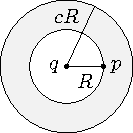
\includegraphics[width=0.3\linewidth]{tikz/nearest_neighbour.pdf}
    \caption{In the $cR$-approximate nearest neighbour problem some point within $cR$ is accepted, if there exists a point $p$ where $d(p,q) \leq R$.}
    \label{fig:nearest_neighbour}
\end{figure}

\subsection{Locality-Sensitive Hash Functions} \label{subsec:locality-sensitive-hashes}

Introduced by Indyck and Motwani in 1998 \cite{indyk_approximate_1998} as an algorithm that solves the approximate nearest neighbour problem (ANN), locality-sensitive hashing (LSH) has since been extensively researched and is now considered among the state of the art for approximate searches in high-dimensional spaces.\footnote{See \cite{nagarkar2021exploring} for an exhaustive survey of NN-Search Techniques.} The basic idea of the approach is to partition the input data using a hash function that is sensitive to the location of the input within the metric space. This way, similar inputs collide with a higher probability than inputs that are far apart. Thus, LSH exhibits fundamental differences to conventional hash functions \footnote{In the following, cryptographic and non-cryptograhpic hash functions are referred to as conventional hashing.}, although the most general definition applies to both.

A hash function is a function that maps a large input set to a smaller target set. The elements of the input set are called \textit{messages} or \textit{keys} and may be of arbitrary different lengths. The elements of the target set are called \textit{digests} or \textit{hash values} and are of fixed size length.

More specifically, we define a hash function as $h: A \rightarrow B : \bm{p} \mapsto \bm{u}$ where $A \subset \mathbb{R}^d$ with $d \in \mathbb{N}$ is the input set and $B=\{0, 1\}^k$ with $k \in \mathbb{N}$ the target set of all bit sequences of fixed size $k$, with $k < d$. According to the notation in \cite[256]{cormen2022introduction}, a hash table is defined by a hash function $h$, that maps the keyspace $K$ into the slots of a hash table $T[0 \,.\,.\, S-1], S \in \mathbb{N}$, i.e. $h: K \rightarrow \{0, 1, \dots, S-1\}$ with $S \ll |K|$. Thus, a message with key $k \in K$ hashes to slot $h(k)$. Additionally, $h(k)$ is the hash value of the key $k$.


% 1. Give formal definitions of Hash function and Hash table
% 2. Explain the difference of conventional hash function and LSH
% 3. Explain the big picture of the algorithm
%%%%%%%%%%%%%%%%%%%%%%%%%%%%%%%%%%%%%%


Typically, conventional hashing is used for the realization of, e.g. hash tables, data integrity checks, error correction methods or database indexes. Depending on the application, different requirements are imposed on the utilized hash function. In this context, the most important property of a hash function is the probability of a \textit{collision}. A collision occurs when two keys $\bm{p}_1 \neq \bm{p}_2$ are projected onto the same hash value $\bm{u} = h(\bm{p}_1) = h(\bm{p}_2)$. For example, cryptographic hash functions are used in systems, where adversaries try to break such systems. Thus, different security requirements are defined for cryptograhpic hash functions \cite[349]{williamcryptography}. In particular, these hash functions are designed to be resistant against collisions, which is the key difference to LSH. Applications that do not require the hash function to be resistant against adversaries, e.g. hash tables, caches or de-duplication, are usually implemented by using a hash function that exhibits relaxed guarantees on the security properties in exchange for significant performance improvements. However, locality-sensitive hashes behave differently as illustrated in Figure \ref{fig:hashing_differences}. LSH projects similar inputs onto the same or near elements. In contrast, conventional hashing tries to distribute projections onto the elements of the target as randomly as possible.

\begin{figure}[t!]
    \centering
    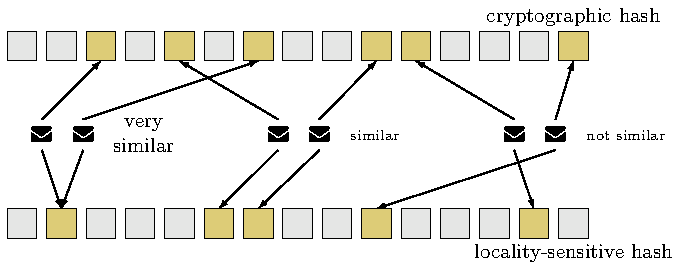
\includegraphics[width=0.8\linewidth]{tikz/hashing_differences.pdf}
    \caption{The behaviour of conventional hashing and LSH}
    \label{fig:hashing_differences}
\end{figure}




%%%%%%%%%%%%%%%%%%%%%%%%%%%%%%%%%%%%%%


% explain the idea of LSH (reduce the search space and then pick a random p or do a linear scan within the reduced search space)

As a locality-sensitive hashing function can be constructed as a general concept, specific families of functions can be derived. We refer to a \textit{family} of hash functions $\mathcal{H}: A \rightarrow B$ as a collection of hash functions that have the same domain and range, share a basic structure and are only differentiated by constants. Three basic requirements are demanded for such a family of functions \cite[99]{leskovec_rajaraman_ullman_2014}.

\begin{enumerate}
    \item Close pairs of input should be hashed in to the same bucket with higher probability than distant pairs.
    \item Specific functions of a family need to be statistically independent, such that the FPR and FNR can be improved by combining two or more functions.
    \item Functions need to be efficient, i.e., be faster compared to an exhaustive search.

\end{enumerate}

The first step is to define LSH generally. Applied on the $cR$-ANN, the first requirement states, with high probability, two points $p$ and $q$ should hash to the same hash value if their distance is at most $R$, i.e., $d(p,q) \leq R$. And if their distance is at least $cR$, the points should hash to different hash values, i.e. $d(p,q) > cR$. Thus,  A formal definition of a locality-sensitive hash function is given as follows \cite{andoni2006near}.

\begin{definition}[Locality-Sesitive Hash Function]
    Given a target distance $R \in \mathbb{R}, R>0$, an approximation factor $c \in \mathbb{R}, c>1$ and probability thresholds $P_1, P_2 \in \mathbb{R}$, a family $\mathcal{H} = \{h: A \rightarrow B$\} is called $(R, cR, P_1, P_2)$-sensitive if for any two points $p,q \in A$ and any hash function $h$ chosen uniformly at random from $\mathcal{H}$ the following conditions are satisfied:
        \[
        \setlength\arraycolsep{0pt}
        \renewcommand\arraystretch{1.2}
            \begin{array}{LCL}
                d(p,q) \leq R & \implies & P[h(p)=h(q)] \geq P_1, \\
                d(p,q) \geq cR & \implies & P[h(p)=h(q)] \leq P_2.
            \end{array}
        \]
\end{definition}
 
Ideally, the gap between $P_1$ and $P_2$ should be as big as possible as depicted in Figure \ref{subfig:exact_probability}, which in fact represents an exact search. This is, as already discussed, no option due to its time and space requirements. Considering a single locality-sensitive function as shown in Figure \ref{subfig:lsh_probability}, where the probability gap between $P_1$ and $P_2$ is relatively close, the false negative rate would be relatively high. Increasing the gap would require to increase $c$ and lead to a high number of false positives. Therefore, a single function would provide only a tradeoff. But it is possible to increase $P_1$ close to $1$ and decrease $P_2$ close to $1/n$ while keeping $R$ and $cR$ fixed as shown in Figure \ref{subfig:lsh_probability_boosted} by introducing a process called \textit{amplification}. Two different forms, namely the AND-construction and the OR-construction, can be applied.

\begin{figure}
    \centering
    \begin{subfigure}[b]{0.3\textwidth}
        \centering
        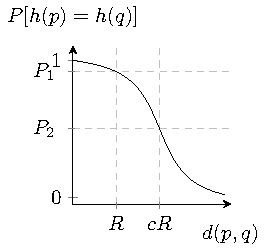
\includegraphics[width=\textwidth]{tikz/lsh_probability.pdf}
        \caption{Single LSH Function.}
        \label{subfig:lsh_probability}
    \end{subfigure}
    \hfill
    \begin{subfigure}[b]{0.3\textwidth}
        \centering
        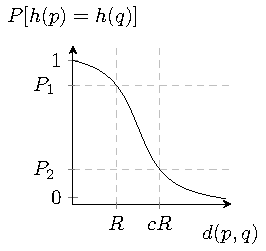
\includegraphics[width=\textwidth]{tikz/lsh_probability_boosted.pdf}
        \caption{Amplified LSH Function.}
        \label{subfig:lsh_probability_boosted}
        \end{subfigure}
        \hfill
        \begin{subfigure}[b]{0.3\textwidth}
            \centering
            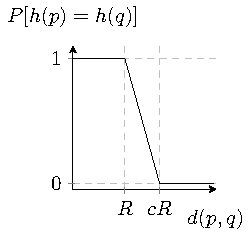
\includegraphics[width=\textwidth]{tikz/exact_probability.pdf}
            \caption{Exact Search}
            \label{subfig:exact_probability}
    \end{subfigure}
    \caption{The behaviour of a $(R, cR, P_1, P_2)$-sensitive function in (\ref{sub@subfig:lsh_probability}) and (\ref{sub@subfig:lsh_probability_boosted}) (adapted from \cite[100]{leskovec_rajaraman_ullman_2014}) approaching the ideal probability gap in (\ref{sub@subfig:exact_probability}) resembling the behaviour of an exact search.}
    \label{fig:lsh_probability}
\end{figure}
   
By applying a logical AND-construction on $\mathcal{H}$ the threshold $P_2$ is reduced. For that, sample $K$ hash functions indepedently from $\mathcal{H}$ and hash each point $p \in P$ to a $K$-dimensional vector with a new constructed function $g \in \mathcal{H}^K$ as

\begin{equation}\label{eq:or_construction}
    g(p) = [h_1(p), h_2(p), \dots, h_K(p)].
\end{equation}

Since all hash functions $\{h_1, \dots, h_K\} \in \mathcal{H}$ are statistically independent the product rule applies and for any two points $p$ and $q$, a collision occurs if and only if $h_i(p)=h_i(q)$ for all $k \in \{1, \dots, K\}$. The probability gap is then defined as follows:

\begin{align}
    P[h_i(p)=h_i(q)] \geq P_1 \implies P[g(p)=g(q)] \geq P_1^K \\
    P[h_i(p)=h_i(q)] \leq P_2 \implies P[g(p)=g(q)] \leq P_2^K.
\end{align}

Thus, by increasing $K$ the threshold $P_2$ can be arbitrarily decreased and approaches zero. However, the AND-construction lowers both $P_1$ and $P_2$. In order to improve $P_1$, the OR-construction is introduced. For that, a number of $L \in \mathbb{N}$ functions $\{g_1, \dots, g_L\}$ are constructed, where each function $g_l, \; l \in \{1, \dots, L\}$ stems from a different family $\mathcal{H}_l$. Note, that the algorithm is successful, when the two points $p, q$ collide at least once for some $g_l$. Therefore, hashing a point $p \in P$ with each $g_l$ results in the following probability for collision.

\begin{align}
    P[\exists l, g_l(p)=g_l(q)] &= 1 - P[\forall l, g_l(p) \neq g_l(q)] \\
                                &= 1 - P[g_l(p) \neq g_l(q)]^L \\
                                &\geq 1 - (1-P_1^K)^L
\end{align}

As the AND-construction lowers both $P_1$ and $P_2$, similarly the OR-construction rises both thresholds. By choosing $K$ and $L$ judiciously, $P_2$ approaches zero while $P_1$ approaches one. Both constructions may be concatenated in any order to manipulate $P_1$ and $P_2$. Of course, the more constructions are used and the higher the values for the parameters $K$ and $L$ are picked, the more time is considered for the application of the function. 

The general algorithm for solving the $cR$-ANN using LSH consists of two consecutive steps. First, a set of points is required for the construction of the data structrue as described in Algorithm \ref{alg:lsh_preprocess}. For each function $g_l$ a corresponding hash table $T_l$ is initialized that will store all data points $p_n$. In other words, all data points are preprocessed and stored $L$ times.The resulting data structure represents the database, which is searched through, when answering a query. Note, that a common collision handling method, such as seperate chaining for example, is applied if a certain slot is already occupied. 

\begin{algorithm}
    \caption{LSH Preprocessing}
    \label{alg:lsh_preprocess}
    \algsetup{indent=2em}
    \begin{algorithmic}[1]
        \REQUIRE $N$ points $p_n \in P$ with $n \in \{1, \dots, N\}, N \in \mathbb{N}$
        \ENSURE data structure $\{T_1, \dots, T_L\}$
        \STATE construct hash functions $g_1, \dots, g_L$ each of length $K$ (see Equation \ref{eq:or_construction})
        \FORALL{$g_l \in \{g_1, \dots, g_L\}$}
            \STATE $T_l \leftarrow$ new HashTable
            \FORALL{$p_n \in P$}
                \STATE add $p_n$ to $T_l[g_l(p_n)]$
            \ENDFOR
        \ENDFOR
    \end{algorithmic}
 \end{algorithm}

 Answering a query point $q$ is done by hashing it multiple times for each $g_l$ as in the preprocessing step (see Algorithm \ref{alg:lsh_query}). Each time, a set of points $P$, stored in the correspoding hash table $T_l$ at the slot $g_l(q)$, are retrieved. That is, identify all $p_n$, such that $g_l(p_n) = g_l(q)$. For each identified $p_n$, a distance function evaluates if the distance $d(p_n, q)$ is within the search perimeter $cR$. If positive, the point is added to the result set $S$, which is returned at the end of the algorithm.

 \begin{algorithm}
    \caption{LSH Query}
    \label{alg:lsh_query}
    \algsetup{indent=2em}
    \begin{algorithmic}[1]
        \REQUIRE a query point $q$ and data structure $\{T_1, \dots, T_L\}$
        \ENSURE a set $S$ of nearest neighours of $q$
        \STATE $S \leftarrow \emptyset$
        \FORALL{$g_l \in \{g_1, \dots, g_L\}$}
            \STATE $P \leftarrow T_l[g_l(q)]$
            \IF{$|P| > 0$}
                \FORALL{$p_n \in P$}
                    \IF{$d(p_n,q) \leq cR$}
                        \STATE add $p_n$ to $S$
                    \ENDIF
                \ENDFOR
            \ENDIF
        \ENDFOR
        \RETURN $S$
    \end{algorithmic}
 \end{algorithm}

 With regard to preprocessing, the consideration of space complexity of Algorithm \ref{alg:lsh_preprocess} is interesting, whereas the runtime of Algorithm \ref{alg:lsh_query} is the most relevant when examining the execution of queries. Fortunately, lower bounds on both quantities have been proven in \cite{motwani2006lower}, resulting in the following theorem.

\begin{theorem}
    Let $(X,d)$ be a metric on a subset of $\mathbb{R}^d$. Given a $(R, cR, P_1, P_2)$-locality sensitive hash family $\mathcal{H}$ and write $\rho = \frac{\text{log}(1/P_1)}{\text{log}(1/P_2)}$. Then for $n = |X|$ and for any $n \geq \frac{1}{P_2}$ there exists a solution to the $cR$-ANN with space complexity $O(dn+n^{1+\rho})$ and query time of $O(n^{\rho})$.
\end{theorem}

Therefore, it follows that the query time of LSH can only be sublinear, if $\rho < 1$, which is the case if the inequality $P_1 > P_2$ is satisfied.



\subsection{Random Projection}\label{subsec:random_projection}

This section presents a specific family $\mathcal{H}$ that is locality-sensitive. The algorithm that bases on this family is known as Gaussian Random Projection (GRP). This approach utilizes the cosine similarity of two real vectors in order to determine their similarity. In the course of this section, basic definitions for Cosine Distance and Cosine Similarity are introduced. Then, the individual calculation steps of the approach are specified. Finally, a visual proof verifies that GRP is a form of LSH.

The cosine distance can be applied in euclidean spaces and discrete versions of euclidean spaces \cite[95]{leskovec_rajaraman_ullman_2014}. For two real vectors $p_1$ and $p_2$, the cosine distance between is equal to the the angle between $p_1$ and $p_2$, regardless of the dimensionality of the space. Note, that by applying the arc-cosine function, the result is in the range $[0, 180]$. The following definition formalizes what has been stated so far.

\begin{definition}[Cosine Distance]
    Given two vectors $p_1$ and $p_2$, the cosine distance $\theta(p_1, p_2)$ is the dot product of $p_1$ and $p_2$ divided by their euclidean distances from the origin ($L_2$-norm):
    \begin{equation}
        \theta(\bm{p}_1, \bm{p}_2) = \text{cos}^{-1} \bigg( \frac{\bm{p}_1 \cdot \bm{p}_2}{||\bm{p}_1|| \: ||\bm{p}_2||} \Bigg).
    \end{equation}
\end{definition}

The angle $\theta$ can be normalized to the range $[0, 1]$ by dividing it by $\pi$. This way, the cosine similarity is simply given by the following definition.

\begin{definition}[Cosine Similarity]
    The cosine similarity is computed as
    \begin{equation}
        1- \frac{\theta(\bm{p}_1, \bm{p}_2)}{\pi}
    \end{equation}
\end{definition}

Introduced in \cite{charikar2002similarity}, the GRP is defined as follows. Given a message $\bm{x} \in A = \{x \in \mathbb{R}^D : 0 \leq x \leq 1 \}$ and a randomly selected hyperplane defined as $\bm{M}=(a_{ij}) \in \mathbb{R}^{D \times K}$ where $a \sim \mathcal{N}(0, I)$, a \textit{gaussian random projection (GRP)} aims to (\RomanNumeralCaps{1}) reduce the dimensionality from $D$ to $L$ dimensions and (\RomanNumeralCaps{2}) provide a binary encoding by first projecting $\bm{x}$ onto $\bm{M}$ and subsequently applying the sign function to each element of the result, which can be formalized as

\begin{gather}
    h(\bm{x}) = [h(\bm{x}, a_1), \dots, h(\bm{x}, a_k)] \text{ with } h(\bm{x}, a) = sign(\bm{x}^Ta) \\
    \text{with } sign(x) = \Biggl\{ \begin{array}{lc}
        0 & \text{if } x < 0, \\
        1 & \text{if } x \geq 0.
    \end{array}
\end{gather}

An illistration of a random hyperplane that dissects the three-dimensional space and partitions the data space is given in Figure \ref{subfig:rp_3d}. The resulting digest $h(x)$ is a binary vector $h(\bm{x}) = \bm{u} \in B = \{0, 1\}^l$ that is used as bucket index for storing $\bm{x}$ in a hash table. For any two messages $\bm{x}_1, \bm{x}_2$, the probability of being hashed to the same bucket increases with a decreasing distance, given as

\begin{equation}\label{eq:rp_proba}
    P[h(\bm{x}_1) = h(\bm{x}_2)] = 1 - \frac{\theta(\bm{x}_1, \bm{x}_2)}{\pi}.
\end{equation}

\begin{figure}[b]
    \centering
    \begin{subfigure}[b]{0.45\textwidth}
        \centering
        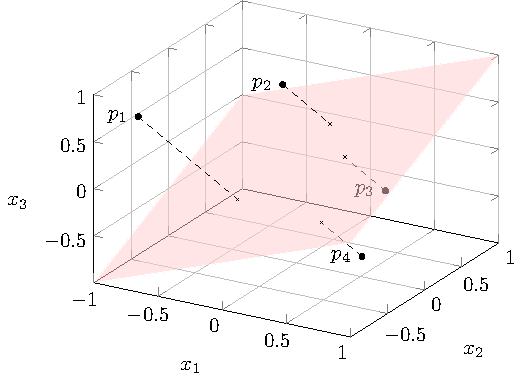
\includegraphics[width=\textwidth]{tikz/random_projection.pdf}
        \caption{Illustration of a random hyperplane (red) partitioning the space.}
        \label{subfig:rp_3d}
    \end{subfigure}
    \hfill
    \begin{subfigure}[b]{0.45\textwidth}
        \centering
        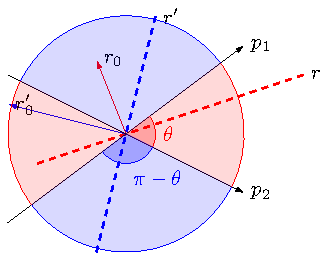
\includegraphics[width=\textwidth]{tikz/random_hyperplane_2d.pdf}
        \caption{Visual Proof of claim in equation \ref{eq:rp_proba}}
        \label{subfig:rp_2d}
    \end{subfigure}
    \caption{}
    \label{fig:random_projection}
\end{figure}

Consider Figure \ref{subfig:rp_2d}, where two vectors $p_1$ and $p_2$, regardless of their dimensionality, define a plane and an angle $\theta$ in this plane.

Pick a hyperplane (actually the normal vector to the hyperplane; hyperplane $v$ is the set of points whose dot product with $v$ is 0)

Hyperplane intersects the plane that is spanned by two vectors $p_1$ and $p_2$ in a line

vector $r_0$ that is normal to the hyperplane represented by the red dashed line; $p_1$ and $p_2$ are on different sides of the hyperplane, thus the projections given by $\langle p_1, r_0 \rangle$ and  $\langle p_2, r_0 \rangle$ will have different signs

vector $r'_0$ that is normal to the hyperplane represented by the blue dashed line;  both $\langle p_1, r'_0 \rangle$ and  $\langle p_2, r'_0 \rangle$ will have the same sign

All angles between the intersection line of the random hyperplane and the plane spanned by $p_1$ and $p_2$ are equally likely. Thus, the probability that the hyperplane looks like the red line is $\theta / \pi$ and like the blue line otherwise.

random projections is a $(R, cR, (1-R/\pi), (1-cR/\pi))$-sensitive family for any $R$ and $cR$. As already explained in Section \ref{subsec:locality-sensitive-hashes}, such a family can be amplified as desired.



% We define a hash function as $h: A \rightarrow B : \bm{p} \mapsto \bm{u}$ where $A \subset \mathbb{R}^d$ with $d \in \mathbb{N}$ is the set of real input data points and $B=\{0, 1\}^l$ with $l \in \mathbb{N}$ the set of all bit sequences of fixed size $l$, with $l < d$. Inputs $\bm{p}$ to hash functions are called \textit{messages} and outputs $\bm{u}$ are called \textit{digests}. 
% A collision occurs when two messages $\bm{p}_1 \neq \bm{p}_2$ are projected onto the same digest $\bm{u} = h(\bm{p}_1) = h(\bm{p}_2)$. We further refer to a \textit{family} of hash functions $\mathcal{H}: A \rightarrow B$ as a collection of hash functions that have the same domain and range, share a basic structure and are only differentiated by constants.

% \subsection{Cryptographic Hash Functions}

% In order to be suitable for cryptographic applications, a hash function $h$ should have, among others, three basic properties. The \textit{first preimage resistance} defines, that for any given $\bm{u} \in B$ it is infeasible to determine any $\bm{p} \in A$ such that $h(\bm{p})=\bm{u}$, allowing $h$ to be effectively one-way only. Furthermore, the \textit{second preimage resistance} defines, that for any given $\bm{p} \in A$ it is infeasible to determine any other $\bm{p}' \in A,\; \bm{p} \neq \bm{p}$ which produces the same output, i.e. $h(\bm{p})=h(\bm{p}')$. Lastly, the \textit{strong collision resistance} states, that is infeasible to determine any two distinct $\bm{p} \neq \bm{p}' \in A$ such that $h(\bm{p})=h(\bm{p}')$.

% \subsection{Non-Cryptographic Hashes} \label{subsubsec:non-cryptographic-hashes}
% Applications that do not require the hash function to be resistant against adversaries, e.g. hash tables, caches or de-duplication, are usually implemented by using a hash function that exhibits relaxed guarantees on the properties defined before in \ref{subsubsec:cryptographic_hashes} in exchange for significant performance improvements.

% \subsection{Locality Sensitive Hash Functions}
% Introduced as an algorithm that solves the $cR$-near neighbour problem, locality-sensitive hashing (LSH) \cite{indyk_approximate_1998} maps similar messages to the same digest with higher probability than dissimilar messages. More formally, given a threshold $R \in \mathbb{R}^{>0}$, an approximation factor $c \in \mathbb{R}^{>1}$ and probabilities $P_1, P_2 \in \mathbb{R}^{\geq 0}$, a family $\mathcal{H}: A \rightarrow B$ is called $(R, cR, P_1, P_2)$-sensitive if for any two points $\bm{p}_1, \bm{p}_2 \in A$ and any hash function $h$ chosen uniformly at random from $\mathcal{H}$ the following conditions are satisfied:

% \begin{itemize}
%     \item if $|| \bm{p}_1 - \bm{p}_2 || \leq R$ then $P[h(\bm{p}_1)=h(\bm{p}_2)] \geq P_1$,
%     \item if $|| \bm{p}_1 - \bm{p}_2 || \geq cR$ then $P[h(\bm{p}_1)=h(\bm{p}_2)] \leq P_2$.
% \end{itemize}

% In order for a $\mathcal{H}$ to be applicable for the $cR$-near neighbour problem, it has to satisfy the inequality $P_1 > P_2$.